\section{La Gestione I/O}
\subsection{Categoria di dispositivi}
Area assai problematica per la progettazione di sistemi operativi perché:
\begin{itemize}
    \item I dispositivi sono molto diversi tra loro
    \item Tante applicazioni che ne fanno uso
    \item Difficili scrivere un SO che supporti tutti i dispositivi
\end{itemize}
le categorie di dispositivi sono:
\begin{itemize}
    \item leggibili dall'utente
    \item leggibili dalla macchina
    \item dispositivi di rete/comunicazione
\end{itemize}
\subsection{Dispositivi leggibili dall'utente}
I dispositivi per la comunicazione diretta ccon l'utente sono:
\begin{itemize}
    \item stampanti
    \item terminali: ovvero monitor + tastiera
    \item joystick
\end{itemize}
\subsection{Dispositivi leggibili dalla macchina}
I dispositivi leggibili dalla macchina sono quelli che soltanto usando l'elettronica si possono leggere, come:
\begin{itemize}
    \item dischi
    \item chiavi USB
    \item Sensori
\end{itemize}
\subsection{Dispositivi di rete/comunicazione}
I dispositivi di rete/comunicazione sono:
\begin{itemize}
    \item schede di rete
    \item modem
    \item WiFI
\end{itemize}
\subsection{Funzionamento(Semplificato) dei dispositivi}
\subsubsection*{input}
Un dispositivo di input prvede di essere interrogato sul valore di una certa grandezza fisica al suo interno:
\begin{itemize}
    \item tastiera: codice Unicode del tasto premuto
    \item mouse: Coordinate dell'ultimo spostamento effettuato
    \item disco: valore dei bit che si trovano in una certa psoizione al suo interno (questo se é usato come input)
\end{itemize}
Se un processo fa una syscall read su un dispositivo di input vuole conoscere questo dato,per poterlo ovviamente elaborare il processo che
gestisce un edito, una volta saputo quale tasto é stato premuto suolla tastiera, puó fare l'echo del carattere corrispondente.
\subsubsection*{output}
Un dispositivi di output prevede di poter cambiare il valore di una certa grandezza fisica al suo interno:
\begin{itemize}
    \item monitor: Valore RGB di tutti i suoi pixel, oppure quelli che cambiano rispetto alla situazione immediatamente precedente
    \item stampante: PDF o PS di un file da stampare
    \item disco: valore dei bit che devono sovrascrivere quelli che si trovano in una certa posizione al suo interno
\end{itemize}
Un processo che effettua una syscall write su un dispositivo del genere vuole cambiare qualcosa, spesso l'effetto é direttamente visibile all'utente, in altre occasioni
l'effetto é visibile solo usando altre funzionalitá di lettura.

Ci sono quindi, minimalmente, due syscall read e write tra i loro argomenti cé un identificativo del dispositivo da leggere o scriver
per esempio,Unix e Linux hanno i file descriptor.
Se c'é una system call read o write viene sollevata una eccezione di sistema, il kernel prende il controllo e si occupa di fare la lettura o la scrittura,
mentre il processo é blocked e passa ad altro, la parte del kernel che gestisce un particolare dispositivo di I/O é chiamata driver, spesso il
trasferimento si fa con il DMA(Direct Memory Access), il driver scrive direttamente in memoria, senza passare per la CPU.
A trasferimento completato il driver solleva un'interruzione, il kernel prende il controllo e risveglia il processo che aveva fatto la syscall,
l'operazione potrebbe anche fallire, (bad block su disco\ldots), potrebbe anche essere necessario fare ulteriori trasferimenti, per esempio
dalla RAM dedicata al DMA a quella del processo.
\subsection{Differenze tra dispositivi di I/O}
I dispositivi di I/O possono differire sotto molti aspetti:
\begin{itemize}
    \item data rate (frequenza di accettazione/emissione di dati)
    \item applicazione
    \item difficolta ne controllo (Tastiera vs disco)
    \item unitá di trasferimento dati (caratteri vs. blocchi)
    \item rappresentazione dei dati
    \item condizioni di errore
\end{itemize}
\subsubsection*{Data Rate}
\begin{figure}[H]
    \centering
    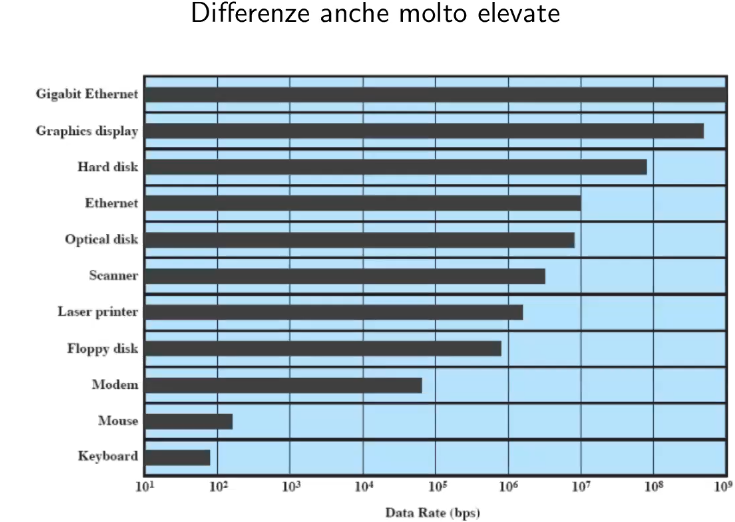
\includegraphics[width=0.5\textwidth]{immagini/DataRate}
    \caption{Data Rate}
\end{figure}
I data rate possono variare di molto, ci sono dispositivi che sono molto lenti, ed altri molto veloci, vediamo per esempio
che il dispositivo gigabit ethernet puó trasferire 10^9 bit al secondo.
\subsubsection*{Applicazioni}
I dischi sono usati per memorizzare files, richiedono un software per la gestione dei file, i dischi sono usati anche per la memoria
virtuale, per la quale serve altro software apposito (nonché hardware), Un terminale usato da un amministratore di sistema dovrebbe
avere una prioritá piú alta.
\subsubsection*{Complessitá di controllo}
Una tastiera o un mouse richiedono un controllo molto semplice, mentre una stampante é piú complicata, ma non troppo, alle stampanti moderne basta ricevere un PDF o PS
la traduzione da PDF ad azioni della stampante é ovviamente complessa, il disco é molto piú complesso, richiede sia un controllo software che hardware
\subsubsection*{Unitá di trasferimento dati}
I dati possono essere trasferiti in unitá di trasferimento divers:
\begin{itemize}
    \item Blocchi di byte di lunghezza fissa (dischi,chiavi USB,CD)
    \item Come un flusso (Stream) di byte, o equivalentemente di caratteri (Qualsiasi cosa non sia memoria secondaria)
\end{itemize}
\subsubsection*{Rappresentazione dei dati}
I dati sono rappresentati secondo codifiche diverse, una vecchia tastiera ad esempio potrebbe rappresentare i suoi dati
in ASCII, una moderna invece utilizza UNICODE, inoltre possono anche essere diversi i controlli di paritá.
\subsubsection*{Condizioni di errore}
La natura degli errori varia di molto da dispositivo a dispositivo, ad esempio nel modo in cui gli errori vengono notificati,
sulle loro conseguenze (fatali/ignorabili).su come possono essere gestiti.
\subsection{Tecniche per effettuare l'I/O}
\begin{figure}[H]
    \centering
    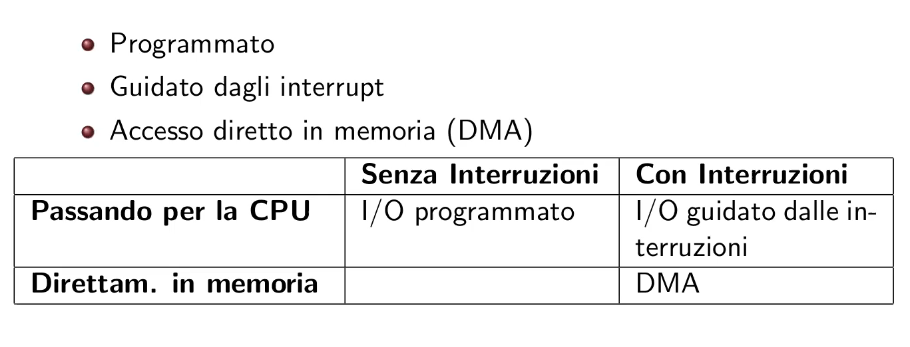
\includegraphics[width=0.5\textwidth]{immagini/TecnicheI_O}
    \caption{I/O}
\end{figure}
Per fare input output ci sono 4 modalitá con o senza interruzioni, con o senza CPU, fare I/O senza interruzzioni significa
fare I/O Programmato, invece usando le interruzzioni si puó fare I/O usando comunque la CPU, oppure evitare di usare la CPU e delegare
il DMA di fare il trasferimento.
\subsubsection*{DMA}
\begin{figure}
    \centering
    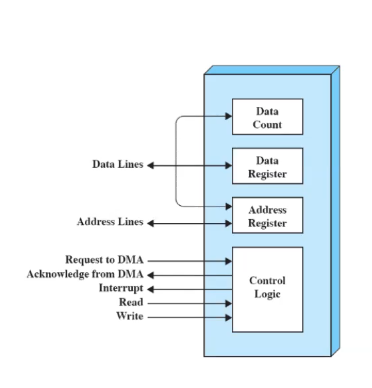
\includegraphics[width=0.5\textwidth]{immagini/DMA}
    \caption{DMA}
\end{figure}
Il DMA contiene una serie di registri che si occupano di contenere i dati da trasferire, poi c'é la control logic
che si occupa di gestire il trasferimento, in pratica si interfaccia con il sistema operativo.
\subsubsection*{Evoluzione della funzionalitá di I/O}
\begin{enumerate}
    \item il processore controlla il dispositivo, il trasferimento é fatto dalla CPU
    \item Viene aggiunto uyn modulo di I/O , direttamente sul dispositivo (I/O programmato) ma senza interrupt ma il processore non si deve occupare di alcuni dettagli del dispositivo stesso
    \item Modulo o controllore di I/O con interrupt, il processore viene avvisato quando il trasferimento é completato
    \item DMA dispositivi comunicano direttamente con la memoria, il processore non é coinvolto
    \item Il modulo I/O diventa un processore separato, il processore "principale" comanda al processore di I/O di eseguire un certo programma di I/O in memoria principale
    \item Processore per l'I/O ha una sua memoria dedicata usata per la comunicazione con terminali interattivi
\end{enumerate}
\subsection{Obbiettivo per SO : Efficienza}
La maggior parte dei dispositivi di I/O sono molto lenti rispetto alla memoria principale, grazie alla multiprogrammazione, alcuni
processi potrebbero essere in attesa del completamento di un'operazione di I/O mentre altri processi sono in esecuzione, Ma l'I/O potrebbe comunque
non tenere il passo con il processore
\begin{itemize}
    \item quindi il numbero di processi ready si riduce fino a diventare 0
    \item  quindi si potrebbe pensare che sia sufficiente portare altri processi ready ma sospesi in memoria principale (Medium-Term Scheduler) , ma anche questa é una operazione di I/O.
\end{itemize}
 si rende quindi necessario
cercare soluzioni software dedicate, a livello di SO, per l'I/O, in particolare per il disco.
\subsection{Obbiettivo per SO : Generalitá}
Per semplicita e per evitare errori, sarebbe bene gestire i dispositivi di I/O in modo uniforme, per esempio esiste un
unica systemcall read che prende il giusto argomento per sapere quale dispositivo leggere, occorre nascondere la maggior
parte dei dettagli dei dispositivi di I/O nelle procedure di basso livello, Progettare le funzioni di I/O in modo modulare
e gerarchico(anche se é difficile farlo in modo generale), le funzionalitá da offrire sono:
\begin{itemize}
    \item read
    \item write
    \item lock
    \item unlock
    \item open
    \item close
\end{itemize}
\subsubsection*{Progettazzione Gerarchica}
Per mantenere la generalitá, si fa uso della progettazione gerarchica, in pratica ci sono dei livelli, che sono usati
all'interno del codice del SO, l'idea é che ogni livello si basa su quello che fa il livello sotto-stante, e quello sottostante
quindi si occupa di fornire servizi a quello soprastante,ogni livello contiene funzionalitá che sono simili per complessitá, tempi di esecuzione
per l'I/O, ci sono 3 macro tipi.
\subsubsubsection*{Dispositivo Locale}
\begin{figure}[H]
    \centering
    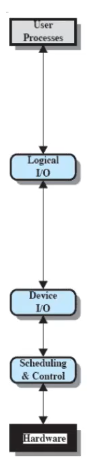
\includegraphics[width=0.2\textwidth]{immagini/DispositivoLocaleI_O}
    \caption{Dispositivo Locale}
\end{figure}
Cose che vengono attaccate direttamente al computer, il livello piú alto é un processo untente, infondo
invece troviamo l'hardware, in mezzo invece troviamo quello che deve fare il sistema operativo, vicino all'hardware troviamo operazioni
di scheduling e controllo ad esempio tanti processi che cercano di scrivere sul monitor, quindi il sistema operativo
deve essere in grado di gestire queste richieste ed ordinarle in modo da non creare conflitti, piú in su troviamo
Device I/O e Logical I/O servono a fornire una interfaccia semplice all'utente, ad esempio logical I/O prende delle richieste
di alto livello ad esempio \textbf{open} e \textbf{close} mentre Device I/O si occupa di trasformare le richieste logiche in comandi.
\subsubsection*{Dispositivo di comunicazione}
\begin{figure}[H]
    \centering
    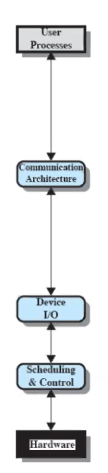
\includegraphics[width=0.2\textwidth]{immagini/Dispositivo di comunicazione}
    \caption{Dispositivo di comunicazione}
\end{figure}
IL dispositivo di comunicazione é praticamente lo stesso del dispositivo locale, solo che é presente un blocco di comunication architecture
\subsubsection*{File System}
\begin{figure}[H]
    \centering
    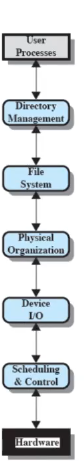
\includegraphics[width=0.2\textwidth]{immagini/FileSystemIO}
    \caption{File System}
\end{figure}
Quello che differisce il file system é che il logical I/O é che sono presenti piú blocchi tra lo user e l'hardware:
\begin{itemize}
    \item Directory Management permette di definire tutte le operazioni che hanno a che fare con i file creare file ecc
    \item File System é la struttura logica che permette di aprire chiudere leggere scrivere ecc
    \item Physical Organization é la struttura che permette di allocare e di-allocare spazio sul disco quindi il sistema operativo interroga il disco per capire dove c'é spazio libero
\end{itemize}
\subsection{Buffering I/O}
Per cercare di rendere piú efficiente il sistema di I/O, é conveniente fare buffering, ovvere tenere in memoria i dati
per completare una certa operazione, essenzialmente l'idea é che noi sappiamo che  le pagine devono essere spostate
dalla memoria principale a disco, e quindi il semplice fatto di usare la memoria virtuale ha come effetto collaterale
gestire I/O, c'é un problema con il DMA, perche un processo puó richiedere un I/O su una certa zona di memoria (DMA), ma viene
swappato subito, Il problema é quindi che ci ritroviamo con 2 richieste discordanti, perché per completare I/O il processo deve essere in
memoria, invece se il sistema operativo swappa il processo questo ha come effetto che bisogna fare essenzialmente l'oppopsto, per riassumere
\textbf{Ci troviamo in una situazione dove la richiesta I/O é in conflitto con la gestione dei processi in memoria}
questo problema é risolvibile con il frame blocking, semplicemente le pagine che vengono accedute dal DMA non possono venire
swappate, tuttavia se inizio a fare troppo frame blocking, limito il numero dei processi che posso eseguire, portando a minore
multiprogrammazzione, Una possibliitá é quella di fare il buffering in memoria, quindi fare I/O on demand, ovvero fare I/O solo quando
viene richiesto, oppure fare buffering in memoria, ovvero fare I/O in anticipo, ovvero fare I/O prima che venga richiesto.
\begin{figure}[H]
    \centering
    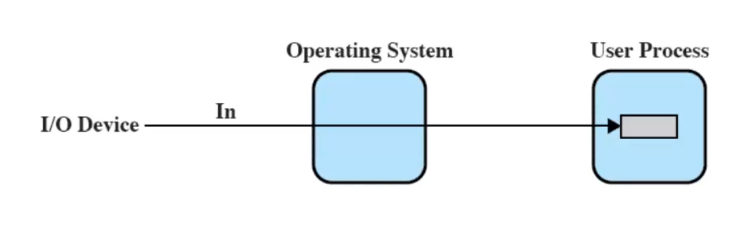
\includegraphics[width=0.5\textwidth]{immagini/I_OSenzaBuffer}
    \caption{senza buffer}
\end{figure}
Senza buffer il sistema operativo dice al dispositivo di I/O di scrivere, e come si vede
il DMA viene istruito di scrivere direttamente nel processo.
\begin{figure}[H]
    \centering
    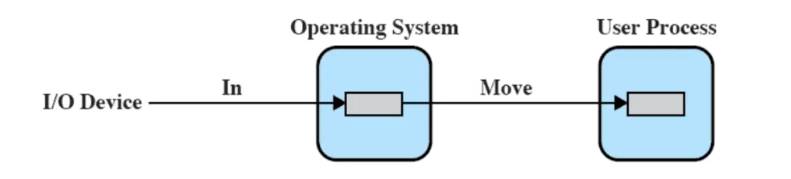
\includegraphics[width=0.5\textwidth]{immagini/I_OConBuffer}
    \caption{Con buffer}
\end{figure}
Con il buffer non operiamo piú direttamente sul processo, ma sul buffer, ovvero una memoria intermedia del sistema operativo,
dove solo in un secondo momento il processo legge i dati, in questo modo si fa un trasferimento da RAM a RAM.
\subsubsection*{buffer singolo orientato ai blocchi}
I trasferimenti di input sono fatti al buffer in system memory, e il blocco viene mandato nello spazio utente quando necessario,
il prossimo blocco viene comunque letto nel buffer,l ínput quindi viene anticipato, i dati, solitamente, vengono acceduti sequenzialmente:
c' é buona probabilitá che servirá,e sará giá stato letto, invece l'output viene posticipato, per questo serve la system call flush\ldots
potrebbe succedere che debuggando un programma, il programma crasha, quello che si fa quindi é fare delle richieste di printf per
vedere se effettivamente il programma passa da quel punto, se non vedo una certa printf, allora il programma crasha prima, ma
questa cosa potrebbe essere non vera a causa del buffering, per questo si usa la system call flush per forzare il buffer a scrivere
\subsubsection*{buffer singolo orientato agli stream}
I terminiali tipicamente hanno a che fare con linee, in questo caso la bufferizzazione riguarda le linee, quindi si bufferizza una
linea intera di input o di output un byte alla volta per i device in cui un singolo carattere premuto va gestito
\subsubsection*{Buffer Doppio}
\begin{figure}[H]
    \centering
    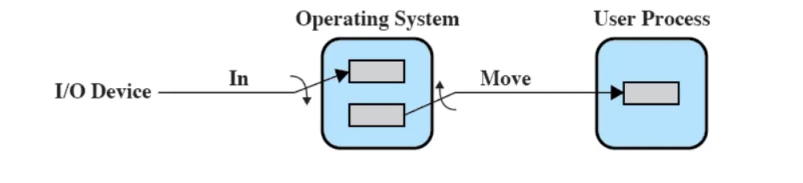
\includegraphics[width=0.5\textwidth]{immagini/bufferdoppioIO}
    \caption{Buffer Doppio}
\end{figure}
Esiste il provlema che nel buffer singolo la zona di memoria dedicata é limitata, quindi esiste la possibilitá che il buffer
si riempa, per ovviare questo problema si puó adottare il buffer doppio.
\subsubsection*{Buffer Multiplo}
\begin{figure}[H]
    \centering
    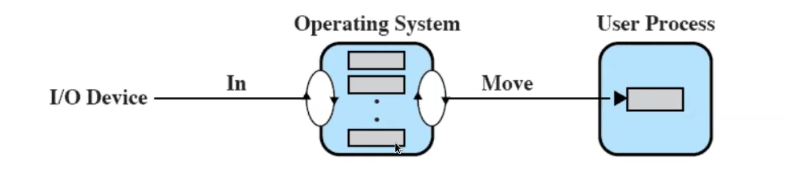
\includegraphics[width=0.5\textwidth]{immagini/BufferMultiplo}
    \caption{Buffer Multiplo}
\end{figure}
In generale si possono avere piú buffer, in pratica un certo dispositivo di I/O ha un puntatore che ha un certo
indirizzo con il buffer da usare, poi il puntatore viene incrementato, e si passa al buffer successivo, in questo modo
quando ho finito di usare l'ultimo riparto dal primo, sicuramente il primo sará libero, progettare questa cosa non é
semplicissima infatti si tratta di un problema che si chiama produttore consumatore
\subsubsection*{pro e contro del buffering}
IL buffering riesce a mantenere il processore non idle anche quando ci sono tante richieste di I/O, quindi ha il compito
di smussare i picchi di richieste di I/O, soprattutto é utile quando ci sono molti e diversi dispositivi da gestire, generalmente
la zona di memoria é statica mentre alcuni SO tipo linux possono decidere di allargarla ai processi.
\subsection{HDD vs SSD}
Abbiamo visto che per gestire l'input output i sistemi operativi devono essere efficienti, ci sono alcune tecniche che devono essere
pensate per alcuni dispositivi in particolare, un di quelli dove c' é stato piú focus sono quelli dell' archivazione di massa,
quindi per aprire un file devo cercare di rispondere nella maniera piú veloce possibile.
\begin{figure}[H]
    \centering
    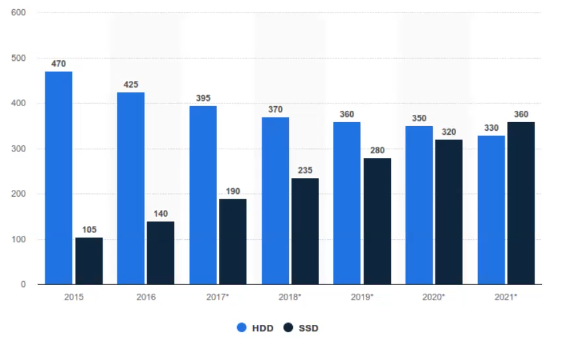
\includegraphics[width=0.5\textwidth]{immagini/HDDvsSDD}
    \caption{HDD vs SSD}
\end{figure}
\subsubsection*{HDD}
\begin{figure}[H]
    \centering
    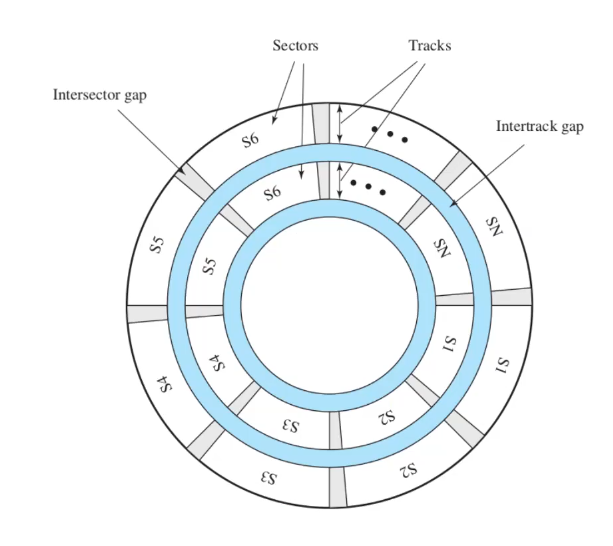
\includegraphics[width=0.5\textwidth]{immagini/schemahdd}
    \caption{HDD}
\end{figure}
Una traccia é un intero percorso (corona circolare), un settore é una parte di una traccia, quindi possiamo
vedere il disco composto da diverse circonferenze che sono allora volta divise in settori, esistono quindi delle
zone di demarcazione per dividere le tracce e i settori, quindi i dati sono sulle tracce essenzialmente
se devo leggere/scrivere devo sapere su quale traccia e settore si trovano, per leggere scrivere é presente un meccanismo
é presente una testina che puó essere una sola o piú testine, esse si spostano/sono posizionate su una traccia , una volta
che sono posizionato sulla traccia se non sono nel giusto settore, il disco deve girare fino a che non si trova nel giusto settore
se i dati sono tanti possono essere su piú settori o addirittura su piú tracce, un settore puó tenere 512 byte
\subsubsection*{prestazioni dell'HDD}
\begin{figure}[H]
    \centering
    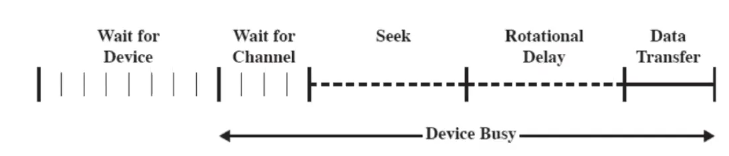
\includegraphics[width=0.5\textwidth]{immagini/tempodiaccessoadisco}
    \caption{Prestazioni HDD}
\end{figure}
Possiamo suddividere il tempo di accesso come nell'immagine :
\begin{enumerate}
    \item Wait for device aspetto che il disco sia pronto e che abbia finito l'operazione precedente
    \item wait for channel aspetto che il canale sia pronto
    \item Seek tempo per muovere la testina fino a posizionare la testina sulla traccia giusta
    \item Rotational delay tempo per far girare il disco fino a che il settore giusto non si trova sotto la testina
    \item Data Transfer tempo per trasferire i dati il disco ruota con la testina che legge, se mi devo spostare si ripartirá da seek
\end{enumerate}
\begin{itemize}
    \item Il tempo di accesso é composto dalla somma di seek e rotational delay
    \item Tempo di trasferimento tempo necessario per trasferire i dati che scorrono sotto la testina
\end{itemize}
\subsubsection*{Politiche di scheduling del disco}
Come é successo per la gestione della ram nel caso in cui siamo su un disco con testine mobili sono stati pensati diversi
algoritmi per rendere piú efficiente la lettura/scrittura.
\subsubsection*{Esmpio generale}
\begin{itemize}
    \item all'inizio la testina si trova sulla traccia numero 100
    \item ci sono 200 tracce
    \item vengono richieste le tracce in ordine : 55,58,39,18,90,160,150,38,184
    \item considereremo solo il seek time, che é il parametro piú importante per le prestazioni
    \item confronteremo con il random scheduling che é il peggiore
\end{itemize}
\subsubsection*{FIFO}
\begin{figure}[H]
    \centering
    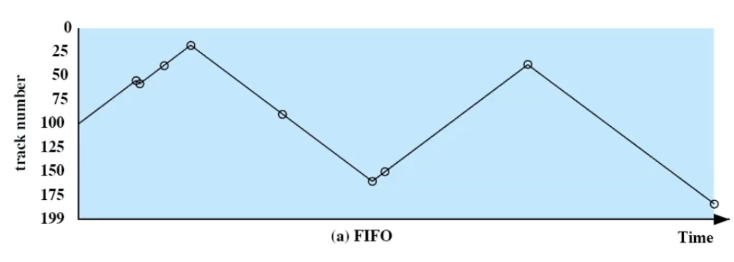
\includegraphics[width=0.5\textwidth]{immagini/FIFOHDD}
    \caption{FIFO}
\end{figure}
Le richieste sono servite in modo sequenziale in questo modo la testina si muove molto,
in questo modo i processi sono serviti in modo equo, se ci sono molti processi in esecuzione, le prestazioni sono
simili allo scheduling random
\subsubsection*{Prioritá}
Esiste la possibilitá di affidarsi alla prioritá dei processi, ovvero lo scopo non é piú quello di migliorare le prestazioni
del disco, ma cerco di soddisfare prima i processi piú importanti, ad esempio i processi interattivi devono essere serviti prima
per garantire l'esperienza utente, i processi lunghi potrebbero aspettare troppo e non va bene per i DBMS
\subsubsection*{LIFO}
Il lifo (si riferisce all'utente) é ottimo per DBMS con transazioni (una sequenza di iterazioni che non puó essere interrotta), il dispositivo é dato all'utente
piú recente, altri utenti quindi posso soffrire di starvation (Continuamente c'é qualcuno che resta fermo) se siamo in un
ambiente con transazioni, se un certo utente ha bisogno di un certo dato, é meglio che questo utente sia servito prima, grafico
non possibile perché per ogni richiesta bisogna sapere quale utente l'ha fatta.
\subsubsection*{Minimo tempo di servizio (SSTF)}
Non vado nell'ordine in cui sono state fatte le richieste, ma le analizzo e cerco di fare in modo di andare
alla traccia piú vicina, in questo modo la testina si muove di meno, quando si esegue questo algoritmo si hanno
un buon numero di richieste, é possibile che ci sia una starvation, perché se arrivano molte richieste vicine (in termini di traccia), quelle
lontane potrebbero non essere servite.
\begin{figure}[H]
    \centering
    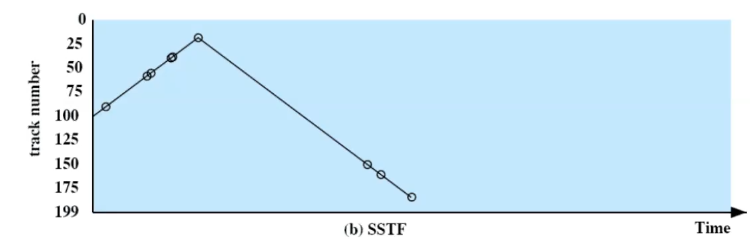
\includegraphics[width=0.5\textwidth]{immagini/MinimoTempoDiServizio}
    \caption{Minimo tempo di servizio}
\end{figure}
\subsubsection*{SCAN}
Per risolvere il problema del minimo tempo di servizio, si puó usare lo SCAN, ovvero le richieste
vengono servite seguendo un solo verso, quando si arriva alla fine si inverte la direzione, in questo modo
si evita la starvation, un problema é che favorisce le richieste vicine ai bordi, perché esse possono essere servite
sia in un veroso che in un'altro, potrebbe anche favorire anche le richieste appena arrivate se queste si trovano sulla stessa
traiettoria 
\begin{figure}
    \centering
    \includegraphics[width=0.5\textwidth]{immagini/SCAN}
    \caption{SCAN}
\end{figure}
\subsubsection*{C-Scan}
Il C-Scan é una variante dello SCAN, in pratica c'é una delle due direzioni della testina che non accetta richieste,
in questo modo il problema delle richieste vicine ai bordi viene risolto.
\begin{figure}[H]
    \centering
    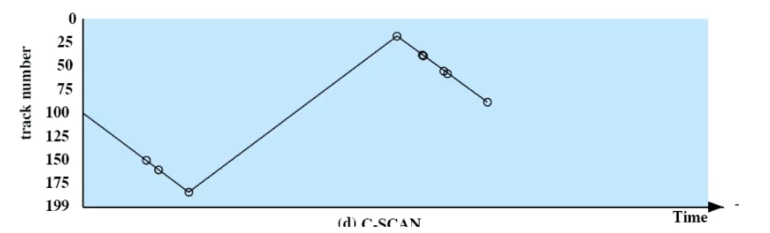
\includegraphics[width=0.5\textwidth]{immagini/C_Scan}
    \caption{C-SCAN}
\end{figure}
\subsubsection*{F-Scan}
Il F-Scan é una variante dello SCAN, in pratica se arrivano nuove richieste le metto in una coda a parte, ad esempi:
ho una coda F (front) e R (rear), l'idea é che scan serve le richieste dentro F, e se arrivano nuove riechieste le
aggiungo a R, quando F é vuota, allora scambio F con R.
\subsubsection*{N-step-SCAN}
L' N-step-SCAN é una variante dello SCAN, in pratica é la generalizzazione dell'F-SCAN, se N é alto, le prestazioni sono
quelle di SCAN, Con N =1 si preferisce comunque usare FIFO.
\subsubsection*{Confronto Prestazioni}
\begin{figure}[H]
    \centering
    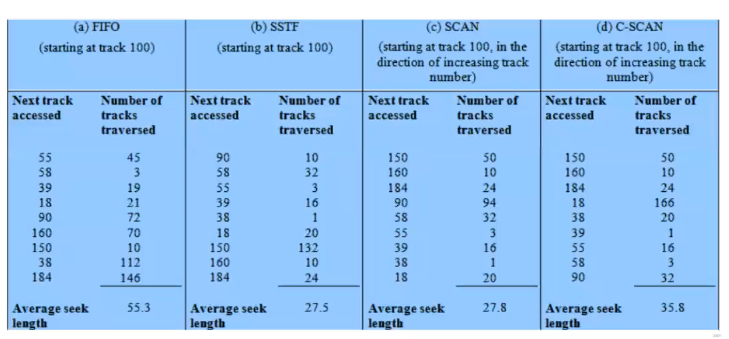
\includegraphics[width=0.5\textwidth]{immagini/ConfrontoSchedulingHDD}
    \caption{Confronto Prestazioni}
\end{figure}
\begin{figure}[H]
    \centering
    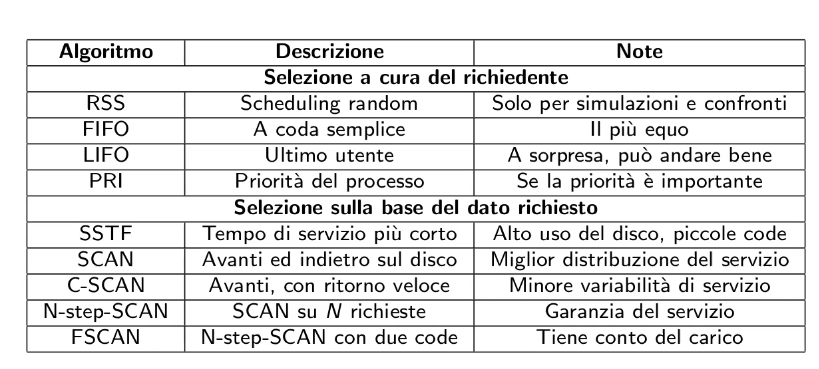
\includegraphics[width=0.5\textwidth]{immagini/RiassuntoAlgoritmiHDD}
    \caption{Confronto Prestazioni}
\end{figure}
\subsectrion{Cache del disco}
La cache del disco anche chiamata page cache é un'altro buffer dedicato al disco, in particolare per alcuni settori,
essenzialmente é una cache quindi contiene una copia di alcuni settori del disco, essendo una cache ha sempre
lo stesso obbiettivo, ovvero prima di andare sul disco si controlla se il dato é presente in cache oppure no, questa
cache é da notare che é situata nella RAM, da notare che questa é una cache software non hardware, non bisogna confonderla
con la cache hardware presente nei dischi, nei dischi moderni quando viene fatta una richiesta i dischi vanno a vedere
la stessa prima di muoversi con la testina.
\subsubsection{Gestione della Cache}
\subsubsection*{Usato meno recentemente (LRU)}
Se occorre rimpiazziare qualche settore nella cache piena, si prende quello nella cache da piú tempo senza referenze,
La cache viene puntatta da uno "stack" di puntatori, quello riferito piú di frequente é quello che sta in cima allo stack,
ogni volta che trovo un settore nella cache, metto in cima il puntatore facendo una operazione di scorrimento, se devo
scegliere quello usato meno di recente, prendo quello in fondo allo stack, in realtá LRU non funzione bene.
\subsubsection*{Least Frequently Used (LFU)}
Piuttosto che usare LRU si preferisce usare LFU, ovvero si tiene traccia di quante volte un settore é stato usato,
quando si deve rimpiazzare un settore, si prende quello usato meno di frequente, ovviamente per implementarlo serve un contatore
per ogni settore che conta quante volte ho fatto l'accesso, l'idea alla base é meno vieni usato meno servi, tuttavia se implementato
in maniera semplice potrebbero esserci effetti collaterali, per esempio puó esistere un settore al quale accedo molte volte
di fila, e poi non lo uso piú, in questo caso il settore non verrebbe mai rimpiazzato.
\subsubsection*{Ibrido LRU-LFU}
Per migliorare la situazione si fa un ibrido tra LRU e LFU, quindi si ha uno stack di puntatori, peró in realtá questo stack
é spezzato in 2 parti con una parte che é nuova ed una che é vecchia, quindi l'idea e che ogni volta ho un riferimento che é nella cache
l'incremetento avviene soltanto se sono nella parte vecchia.
\begin{figure}[H]
    \centering
    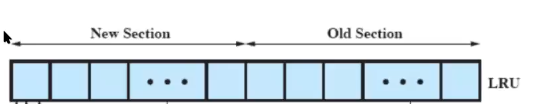
\includegraphics[width=0.5\textwidth]{immagini/IbridoLRU-LFU}
    \caption{Ibrido LRU-LFU}
\end{figure}
Quello rappresentato sopra é lo stack di puntatori quindi punta alla cache, come si vede c'é una parte
nuova e una vecchia, se quello che sta a sinistra é il most recently used, quello che sta a destra é il least recently used
quello che dovrei prendere se usassi LRU standard, quindi se io ho un processo che richiede un settore, che é nella sezione
nuova lo sposto in cima alla sezione ma non incremento il contatore, lo incremento solo se si trovava nella sezione vecchia,
se io ho un miss, carico il settore nuovo con il contatore con valore 1, quindi il vantaggio che se io mi riferisco spesso
ad un settore, nuovo siccome il contatore non viene modificato, posso evitare che nonostante le numerose chiamate in un breve
periodo di tempo, il settore rimanga in memoria perché ha un counter con un valore alto, dalla parte nuova alla parte vecchia
per scorrimento, invece dalla parte vecchia alla parte nuova per riferiment, é da notare che cé ancora un problema se non c'é
presto un riferimento ad un blocco, questo potrebbe essere rimpiazzato, perché i riferimenti a lui non arrivano, abbastanza velocementi
, per esempio io mi riferisco al blocco \textbf{A} ed ha il contatore 1, arrivano altri riferimenti a \textbf{B} e \textbf{C} \ldotsecc
puó succedere che il blocco \textbf{A} venga rimpiazzato, perché i suoi riferimenti tardano ad arrivare e per questo
motivo lui scorre verso la parte vecchia fino ad essere sostituito.
\subsubsection*{Sostituzione Basata su frequenza 3 Segmenti}
Per ovviare al problema dello scorrimento, invece di avere 2 parti, si hanno 3 parti, in questo modo i contatori vengono incrementati
sia nella parte di mezzo che in quella vecchia, per contro si puó rimpiazzare solo nella parte vecchia, per il resto é uguale
a prima, anche se non arriva presto il riferimento la probabilitá di essere sostituito é minore.
\begin{figure}[H]
    \centering
    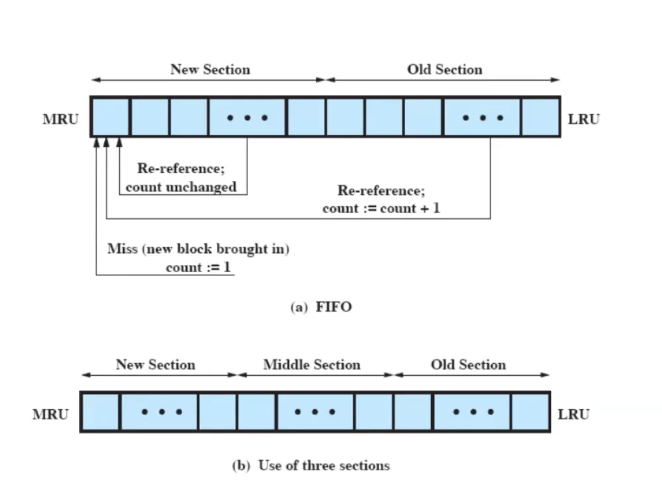
\includegraphics[width=0.5\textwidth]{immagini/sostituzione-3-segmenti}
    \caption{Sostituzione Basata su frequenza 3 Segmenti}
\end{figure}
\begin{figure}[H]
    \centering
    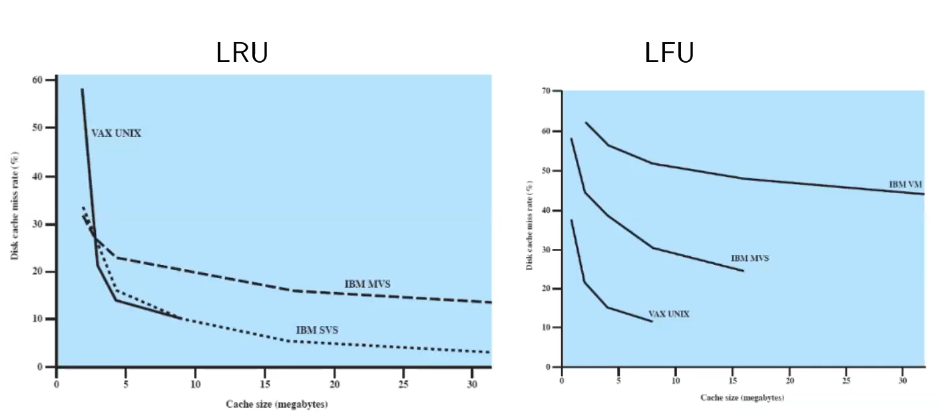
\includegraphics[width=0.5\textwidth]{immagini/RisultatiEsperimentiCacheDisco}
    \caption{Risultati Esperimenti Cache Disco}
\end{figure}
LRU é meglio perché sono studi diversi: se la sequenza é la stessa, conviene usare LFU.
\subsection{RAID}
Un altra cosa importante quando si parla di I/O é il RAID, che significa Redundant Array of Independent Disks, ovvero
un insieme di dischi indipendenti che lavorano insieme, e ci sono diversi modi per farli lavorare insieme, é comunque
possibile trattarli separatamente per esempio, Windows li mostrerebbe esplicitamente come dischi diversi, con etichette diverse
, mentre Linux, si potrebbe dire che alcune directory sono in un disco, altre in un altro, quindi si specifica all'inizio, oppure
si possono considerare diversi dischi fisici come un unico disco logico.
\subsubsection*{Dischi Multipli}
Possibilitá ovvia : Linux LVM (Logical Volume Manager), alcuni files/directory sono memorizzati su un disco, altri su un altro,
ci pensa una parte del kernel, LVM appunto, l'utente puó non occuparsi di decidere dove salvare i file, con la tecnica del mount
di directory divers, potrebbe succedere che una directory cresca fio a riempire il relativo disco, mentre l'altra resta vuota,
LVM é fatto apposta per tenere conto di questo problema.
\subsubsection*{RAID}
L' LVM va bene per pochi dischi, ed in generale se non si é interessati alla ridondanza, questa parte di ridondanza LVM
non la gestisce, per questo esiste il RAID, il RAID era stato pensato per la ridondanza ma con esso si riescono anche a velocizzare
alcune operazioni, esistono device composti da piú dischi fisici gestiti da un RAID direttamente a livello di dispositivo.
\subsubsection*{Dischi RAID : gerarchia}
\subsubsection*{RAID 0}
\begin{figure}[H]
    \centering
    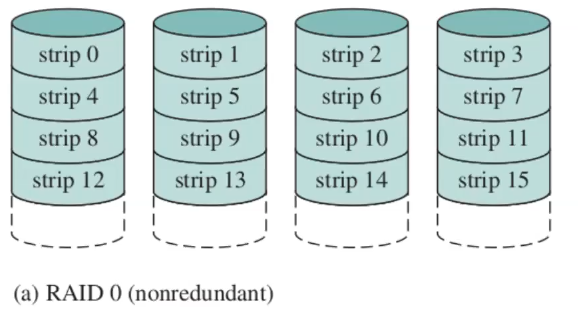
\includegraphics[width=0.5\textwidth]{immagini/RAID0}
    \caption{Dischi RAID}
\end{figure}
Nell'raid 0 i dati sono distribuiti per maggiore efficienza nell'accesso e non c'é ridondanza, perché puó essere parallelo, i dischi sono divisi
in strip, ogni strip contiene un certo numbero di settori, un insieme di strips sui vari dischi (una riga) si chiama stripe.
\subsubsection*{RAID 1}
\begin{figure}[H]
    \centering
    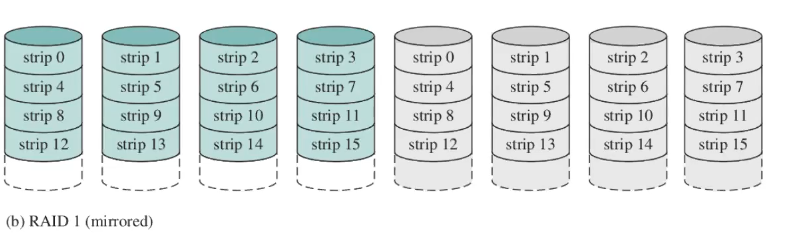
\includegraphics[width=0.5\textwidth]{immagini/RAID1}
    \caption{Dischi RAID}
\end{figure}
Il RAID 1 é come il RAID 0 ma duplicando ogni dato, fisicamente si hanno 2N, ma la
capacitá di memorizzazione é N, in pratica si scrive su entrambi i dischi, se si rompe un disco, sono sicuro di recuperarlo,
se se ne rompono 2 bisogna vedere quali si sono rotti
\subsubsection*{RAID 2}
\begin{figure}[H]
    \centering
    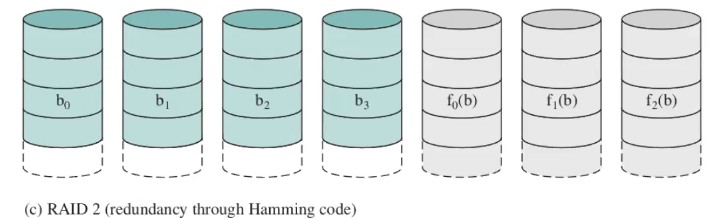
\includegraphics[width=0.5\textwidth]{immagini/RAID2}
    \caption{Dischi RAID}
\end{figure}
Nell'RAID 2 non si usa la copia 1:1  ma si usa la paritá, l'idea quindi é quella che invece di replicare l'intera informazione
utilizzo un opportuno codice di paritá, che serve a correggere i dati, l'overhead é logaritmico
\subsubsection*{RAID 3}
\begin{figure}[H]
    \centering
    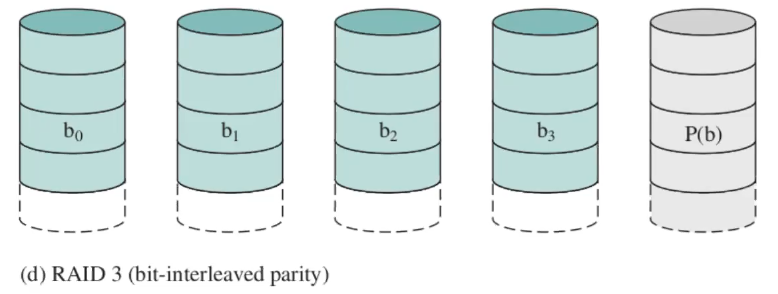
\includegraphics[width=0.5\textwidth]{immagini/RAID3}
    \caption{Dischi RAID}
\end{figure}
Nell'RAID 3 abbiamo un solo disco di overhead, in pratica per ogni bit il disco in piú memorizza la paritá,
comunque resta possibile il recupero dei dati, quando fallisce un unico disco oppure il disco che contiene la paritá.
\subsubsection*{RAID 4}
\begin{figure}[H]
    \centering
    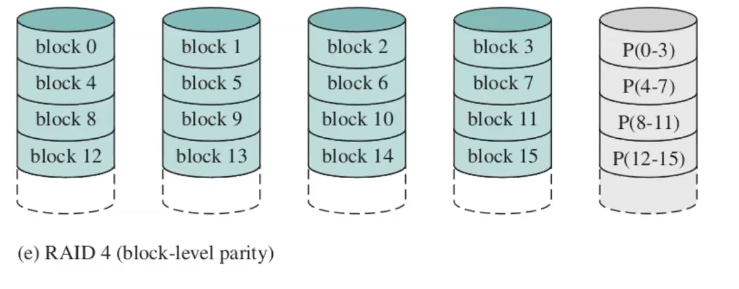
\includegraphics[width=0.5\textwidth]{immagini/RAID4}
    \caption{Dischi RAID}
\end{figure}
Il raid 4 é simile al raid 3, ma invece di funzionare di bit in bit, funziona a livello di blocco.
\subsubsection*{RAID 5}
\begin{figure}[H]
    \centering
    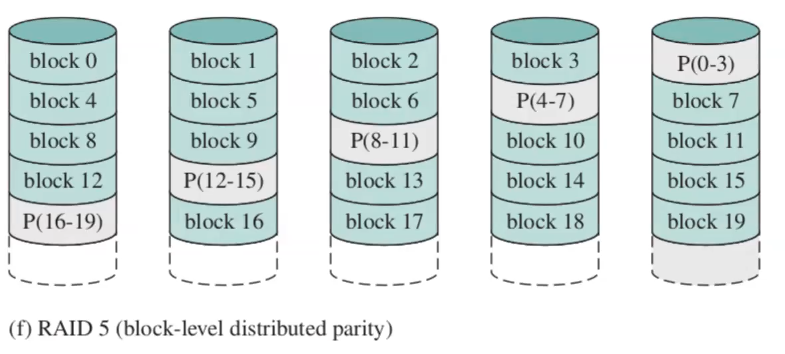
\includegraphics[width=0.5\textwidth]{immagini/RAID5}
    \caption{Dischi RAID}
\end{figure}
Nel RAID 5 la paritá é distribuita su tutti i dischi, in pratica non si ha un disco di paritá, ma la paritá é distribuita
su tutti i dischi, in pratica si ha un disco di paritá virtuale, in questo modo si ha un miglioramento delle prestazioni, permettendo
comunque l'accesso parallelo.
\subsubsection*{RAID 6}
\begin{figure}[H]
    \centering
    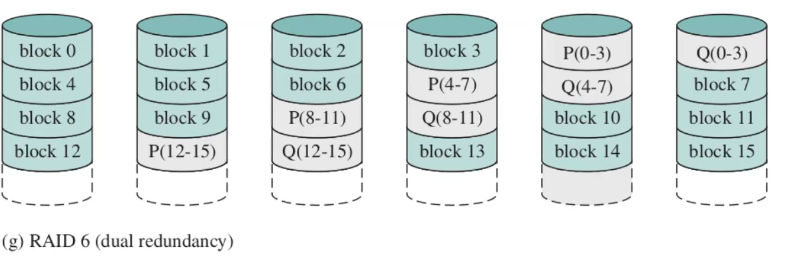
\includegraphics[width=0.7\textwidth]{immagini/RAID6}
    \caption{Dischi RAID}
\end{figure}
Il RAID 6 é simile al RAID 5, ma si hanno 2 dischi di paritá virtuali, in pratica si ha una ridondanza maggiore,
ed é anche possibile recuperare i dati se falliscono 2 dischi, per le operazioni di lettura con il
RAID 5 esiste una somiglianza con il RAID 6 mentre per le operazioni di scrittura il RAID 6 é piú lento.
\subsubsection*{Riassunto}
\begin{figure}[H]
    \centering
    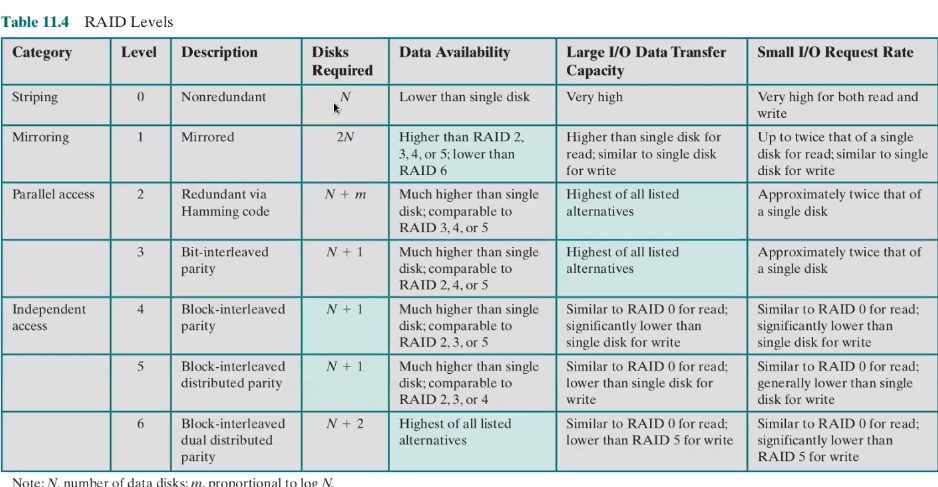
\includegraphics[width=1\textwidth]{immagini/Confronto RAID}
    \caption{Confronto di tutti i RAID}
\end{figure}
é da notate che se faccio una operazione sul RAID, tutti i dischi effettuano in sincrono, un operazione
su un raid é una operazione su un sottoinsieme dei sui dischi, il vantaggio di avere un RAID diverso da 0 é possibile
recuperare i dati se fallisce un disco, smallI/O Request rate descrive il modo come i dischi gestiscono piccole richieste
di \textbf{I/O}
\subsubsection*{I/O Linux}
Linux soprattuto per quanto riguarda la gestione della page cache, la page cache é unica e combatte nella memoria destinata agli utenti per tutti i trasferimenti compresi quelli dovuti alla gestione della memoria
virtuale, questo porta 2 vantaggi : condensare le scritture sul disco siano esse dovute a I/O o alla gestione della memoria virtuale, inoltre
serve anche per sfruttare la localitá dei riferimenti, si scrive sul disco o quando é rimasta poca memoria: una parte della page cache
é ridestinata ad uso diretto dei processi, quando l'etá delle pagine "sporche"  va sopra una certa soglia,
Niente politica separate di replacement:  é la stessa utilizzata per la sostituzione delle pagine (algoritmo dell'orologio).


































































